\documentclass[tikz]{standalone}

\usepackage[T1]{fontenc}
\usepackage[utf8]{inputenc}
\usepackage{eulervm}
\usepackage{amsmath}
\usepackage{bm}
\usepackage{tikz}
\usepackage{environ}

\usetikzlibrary{fit}
\usetikzlibrary{patterns}
\usetikzlibrary{arrows}

\input{./settings/colors}

\begin{document}
  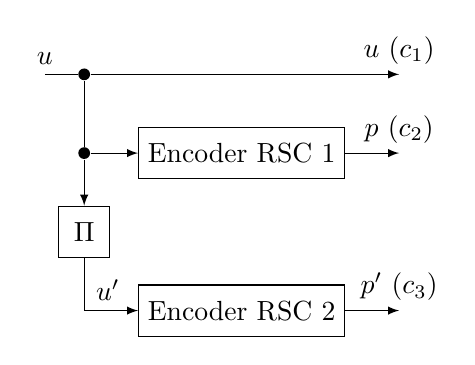
\begin{tikzpicture}%[scale=\tikzscale]
  \tikzset{STA/.style={draw, minimum height=0.65cm, minimum width=0.65cm} }

  \node (d0) at (0.0, 0.0) [circle,fill,inner sep=1.5pt]{};
  \node (d1) at (0.0,-1.0) [circle,fill,inner sep=1.5pt]{};

  \node[STA] (pi) at (0.0, -2.0) {$\Pi$};

  \node[STA] (e1) at (2.0, -1.0) {$\text{Encoder RSC 1}$};
  \node[STA] (e2) at (2.0, -3.0) {$\text{Encoder RSC 2}$};

  \draw[- ,>=latex] (-0.5,0.0) node [left,  above] {$u$} -- (d0);
  \draw[->,>=latex] (d0) -- (+4.0,0.0) node [left,  above] {$u~(c_1)$};
  \draw[- ,>=latex] (d0) -- (d1);
  \draw[->,>=latex] (d1) -- (e1);
  \draw[->,>=latex] (d1) -- (pi);
  \draw[->,>=latex] (pi) |- (e2) node [left, above,xshift=-17mm] {$u'$};

  \draw[->,>=latex] (e1) -- (4.0, -1.0) node [right, above] {$p~(c_2)$};
  \draw[->,>=latex] (e2) -- (4.0, -3.0) node [right, above] {$p'~(c_3)$};
  \end{tikzpicture}
\end{document}